%\setlength{\parindent}{0pt}
\documentclass{article}
\usepackage{amsmath}
\usepackage{amssymb}
\usepackage{amsthm}
\usepackage{latexsym}

\usepackage{amsopn}
\DeclareMathOperator{\stab}{Stab}
\DeclareMathOperator{\perm}{Perm}
\DeclareMathOperator{\im}{im}
\DeclareMathOperator{\Aut}{Aut}
\DeclareMathOperator{\Hom}{Hom}
\DeclareMathOperator{\Perm}{Perm}
\DeclareMathOperator{\Frac}{Frac}
\DeclareMathOperator{\Pic}{Pic}
\DeclareMathOperator{\id}{id}
\DeclareMathOperator{\Tr}{Tr}
\DeclareMathOperator{\Spec}{Spec}
\DeclareMathOperator{\Proj}{Proj}
\DeclareMathOperator{\codim}{codim}


\usepackage[dvipsnames]{xcolor}
 
\definecolor{mypink1}{rgb}{0.858, 0.188, 0.478}

%\usepackage{color}
%\definecolor{keywordcolor}{rgb}{0.7, 0.1, 0.1}   % red
%\definecolor{commentcolor}{rgb}{0.4, 0.4, 0.4}   % grey
%\definecolor{symbolcolor}{rgb}{0.0, 0.1, 0.6}    % blue
%\definecolor{sortcolor}{rgb}{0.1, 0.5, 0.1}      % green
%\usepackage{listings}
%\def\lstlanguagefiles{lstlean.tex} 
%\lstset{language=lean}

\usepackage{enumitem}
\usepackage{tikz-cd}

\usepackage{tikz,tkz-euclide}
\usetikzlibrary{arrows,calc,intersections}
%\usetkzobj{all}

\usepackage{enumitem}
\usepackage[margin=2.2cm]{geometry}

\newcommand{\ideal}{\ensuremath{\triangleleft}}
\newcommand{\ol}{\ensuremath{\overline}}
\newcommand{\p}{\ensuremath{\mathfrak{p}}}
\newcommand{\m}{\ensuremath{\mathfrak{m}}}
\newcommand{\A}{\ensuremath{\mathbb{A}}}
\newcommand{\Z}{\ensuremath{\mathbb{Z}}}
\newcommand{\C}{\ensuremath{\mathbb{C}}}
\newcommand{\R}{\ensuremath{\mathbb{R}}}
\newcommand{\Q}{\ensuremath{\mathbb{Q}}}
\newcommand{\N}{\ensuremath{\mathbb{N}}}
\newcommand{\F}{\ensuremath{\mathbb{F}}}
\renewcommand{\P}{\ensuremath{\mathbb{P}}}
\newcommand{\Ox}{\mathscr{O}}

\newcommand{\q}{\ensuremath{\mathfrak{q}}}
%\newcommand{\N}{\ensuremath{\mathbb{N}}}

\usepackage{mathrsfs}
%\usepackage{fontspec}
%\usepackage{mathtools}
%\usepackage{unicode-math}

\usepackage{natbib}
\bibliographystyle{humannat}
%\bibliographystyle{unsrtnat}
%\bibliographystyle{abbrvnat}

\theoremstyle{definition}
\newcounter{dummy} \numberwithin{dummy}{section}
\newtheorem{lemma}[dummy]{Lemma}
%\newtheorem*{lemma*}[dummy]{Lemma}
\newtheorem{prop}[dummy]{Proposition}
\newtheorem{defi}[dummy]{Definition}
\newtheorem{cor}[dummy]{Corollary}
\newtheorem{example}[dummy]{Example}
\newtheorem{thm}[dummy]{Theorem}



\newcommand*{\DashedArrow}[1][]{\mathbin{\tikz [baseline=-0.25ex,-latex, dashed,#1] \draw [#1] (0pt,0.5ex) -- (1.3em,0.5ex);}}%
\newcommand{\dto}{\DashedArrow[->,densely dashed]}
%\newcommand{\da}{\DashedArrow}

%\usepackage{microtype}
\usepackage[activate={true,nocompatibility},final,tracking=true,kerning=true,spacing=true,factor=1100,stretch=10,shrink=10]{microtype}
\author{Louis Carlin -- u6384109}
\title{World Models with MDRNNs}
\usepackage[pdftex]{hyperref}
\hypersetup{
  colorlinks=true
}
\begin{document}
\maketitle
\begin{abstract}
In World Models (CITEME) David Ha et al describe an architecture allowing a computer agent to learn an internal model of its own environment.
Their model was powerful enough that agents could be trained in its dreamed simulation to achieve good performance in the original environment.
In this project I set out to create my own implimentation of the World Models architecture.

\end{abstract}

\section{Introduction}
%background stuff of other world models
When humans make decisions we often use an internal model of the problem at hand to inform our decision, allowing us to predict or calculate how the world might unfold based on our actions.
This model based approach may be something we are conscious of, as in the case of a chess player who uses their knowledge to look ahead and evaluate potential moves.
It also happens unconsciously, for example with batters in baseball who use an internal model to infer the position of the ball based on the the way the pitcher throws it, rather than reacting to the position of the ball milliseconds before it hits their bat.
In either case this internal model greatly improves our performance at these tasks.

In reinforcement learning we seek to develop computer agents which are capable of \textit{learning} to complete tasks.
Inspired by the success of own model based thought process we naturally seek to equip these agents with models of their environment.
There are several different ways this has been done.
Most traditionally an agent may be supplied with a model which has been handcrafted by a human. %TODO example
Unfortunately models made in this way are usually domain specific and thus the approach requires significant human involvement any time we try adapt an agent to learn in a new environment.
In a complex or partially unobservable environment it may even be infeasible for a human to equip an agent with a model adequately describing its world. %example?
More recently, deep reinforcement learning has circumvented this problem by increasing the complexity of the learned agent.
Agents constructed using architectures such as recurrent neural networks (RNNs) learn to perform complex computations.
In many cases they are able to harness this power to essentially learn their own model of the environment, allowing them to succeed at complex tasks without human intervention.
Deep reinforcement learning is not a complete solution however: training of complex agents is notoriously difficult, with what is known as the \textit{Credit Assignment Problem} often preventing agents from learning in environments with sparse reward signals.
A third approach, championed by Schmidthuber is to decouple the learning process, first learning a model $M$ and then using this model to train a controller $C$. %CITEME
The advantage of this approach is that complex models can be learned without worrying about credit assignment, allowing us to more easily train a comparatively simple controller.

World Models is a particularly simple implimentation of Schmidthuber's approach which has been shown to be remarkable effective at learning in image based environments. %CITEME
It breaks an agent into three components, the first two are vision $V$ and model $M$, and together these allow an agent to interpret and model its world.
The controller $C$ is then trained using both features of the environment and some of the internal knowledge of $M$.
Significantly, the internal model comprised of $V$ and $M$ is powerful enough to recreate a simulated version of the original environment, known as a \textit{dream}.
These dreams were close enough to the original environment that agents could be trained entirely inside a dream to perform well in the original environment.
In this project I primarily set out to investigate this part of World Models, which consists of the $V$ and $M$ components.

The structure of this report is as follows.
We begin with a brief overview of the World Models' architecture which serves as the primary motivation throughout this report.
In the subsequent three sections we discuss some of the theory behind each of the three components of World Models.
Finally, in the last section I discuss my own implementation and results.

\section{The World Models' Architecture}
%\subsection{Problem Description}
World Models uses a fairly standard description of the reinforcement learning problem.
Environments are broken down into discrete time steps.
At a time $t$ an agent receives a partial observation of the environment $o_t$ and are reward $r_t$.
The agent must then choose an action $a_t$ from a set of possible actions.
In an \textit{episodic} task where there are only ever finitely many time steps the agent's task is to pick $a_t$ such that the sum of future rewards is maximised.
In a \textit{continuing} task where the environment is ongoing an agent instead picks $a_t$ to maximise a weighted sum of future rewards where more distant rewards are weighted with decreasing values to ensure the sum converges.

Although Schmidthuber's original ideas apply much more generally the World Models architecture is adapted to image based problems where the observation $o_t$ is a two dimensional image.
Environments such as these are navigated with ease by humans playing videogames, yet still remain a challenge in reinforcement learning.
David Ha et al. empirically tested their model in two different environments.
The first one was \texttt{CarRacing-v0} where an agent must learn to drive a car based on a top-down image of the racing track. %CITEME
Here the agent is rewarded more the more tiles they visit, which incentivises speedier and more accurate driving.
The second environment was \texttt{VizDoom: Take Cover} where an agent learns to dodge fireballs thrown at it by demons in the 3D environment of the videogame Doom.
In this environment observations are first person images from the perspective of the agent and rewards are simply given to the agent based on survival time.
%TODO picture of both environments

\begin{figure}[h]
  \centering
  \begin{minipage}{0.45\textwidth}
      \centering
      \includegraphics[width=0.9\textwidth]{CarRacing-v0.jpeg} % first figure itself
      \caption{An observation from the \texttt{CarRacing-v0} environment}
  \end{minipage}\hfill
  \begin{minipage}{0.45\textwidth}
      \centering
      \includegraphics[width=0.9\textwidth]{VizDoom.jpeg} % second figure itself
      \caption{An observation from the \texttt{VizDoom: Take Cover} environment}
  \end{minipage}
\end{figure}

%overview of model V-M-C
The World Models' architecture is split into three components: \textit{Vision (V), Memory (M)}, and \textit{Controller (C)}.
The Vision component is comprised of an variational autoencoder.
It takes in an image observation $o$ and gives a much smaller vector $z$, known as the \textit{latent representation}, which we can think of as a compressed version of $o$.
The idea behind this compression is that it will be easier to learn an internal model of the dynamics of this smaller latent state than to try predict the evolution of the observation images. 
The Memory component is a Mixture Density Reccurrent Neural Net (MDRNN) and forms the bulk of agent's internal model.
Given the current latent state $z_t$, an action $a_t$, and its own memory output $h_{t}$ from the previous state, $M$ is trained to predict what the next latent state $z_{t+1}$ will be given that action.
That is, $M$ learns the distribution $p(z_{t+1} | z_t, a_t, h_t)$.
Finally, the Controller learns a simple linear mapping from the latent state $z$ and previous memory state $h$ to an action. 

\begin{figure}[h]
  \centering


\tikzset{every picture/.style={line width=0.75pt}} %set default line width to 0.75pt        

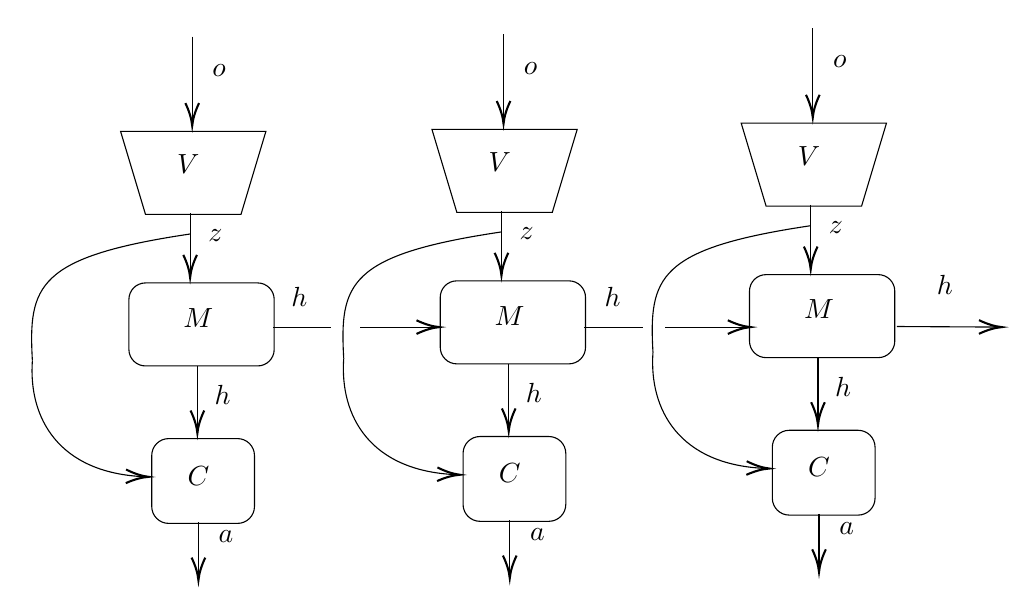
\begin{tikzpicture}[x=0.75pt,y=0.75pt,yscale=-1,xscale=1]
%uncomment if require: \path (0,300); %set diagram left start at 0, and has height of 300

%Shape: Trapezoid [id:dp8835259262509831] 
\draw   (214,73) -- (202,113) -- (156,113) -- (144,73) -- cycle ;
%Rounded Rect [id:dp0285219553359235] 
\draw   (148,154) .. controls (148,149.58) and (151.58,146) .. (156,146) -- (210,146) .. controls (214.42,146) and (218,149.58) .. (218,154) -- (218,178) .. controls (218,182.42) and (214.42,186) .. (210,186) -- (156,186) .. controls (151.58,186) and (148,182.42) .. (148,178) -- cycle ;
%Rounded Rect [id:dp3457403063059383] 
\draw   (159,229.17) .. controls (159,224.66) and (162.66,221) .. (167.17,221) -- (200.33,221) .. controls (204.84,221) and (208.5,224.66) .. (208.5,229.17) -- (208.5,253.69) .. controls (208.5,258.2) and (204.84,261.86) .. (200.33,261.86) -- (167.17,261.86) .. controls (162.66,261.86) and (159,258.2) .. (159,253.69) -- cycle ;
%Straight Lines [id:da5830231307220126] 
\draw    (181,186) -- (181,216.43) ;
\draw [shift={(181,218.43)}, rotate = 270] [color={rgb, 255:red, 0; green, 0; blue, 0 }  ][line width=0.75]    (10.93,-3.29) .. controls (6.95,-1.4) and (3.31,-0.3) .. (0,0) .. controls (3.31,0.3) and (6.95,1.4) .. (10.93,3.29)   ;
%Straight Lines [id:da21875827228445366] 
\draw    (177.5,112.43) -- (177.5,141.43) ;
\draw [shift={(177.5,143.43)}, rotate = 270] [color={rgb, 255:red, 0; green, 0; blue, 0 }  ][line width=0.75]    (10.93,-3.29) .. controls (6.95,-1.4) and (3.31,-0.3) .. (0,0) .. controls (3.31,0.3) and (6.95,1.4) .. (10.93,3.29)   ;
%Curve Lines [id:da18494477060365933] 
\draw    (177.5,122.43) .. controls (103.5,133.43) and (99.5,147.43) .. (101.5,183.43) ;
%Curve Lines [id:da3167428765764193] 
\draw    (101.5,183.43) .. controls (99.53,211.01) and (114.05,237.62) .. (155.58,239.37) ;
\draw [shift={(157.5,239.43)}, rotate = 181.33] [color={rgb, 255:red, 0; green, 0; blue, 0 }  ][line width=0.75]    (10.93,-3.29) .. controls (6.95,-1.4) and (3.31,-0.3) .. (0,0) .. controls (3.31,0.3) and (6.95,1.4) .. (10.93,3.29)   ;
%Straight Lines [id:da13659803234644108] 
\draw    (178.5,27.29) -- (178.5,68.29) ;
\draw [shift={(178.5,70.29)}, rotate = 270] [color={rgb, 255:red, 0; green, 0; blue, 0 }  ][line width=0.75]    (10.93,-3.29) .. controls (6.95,-1.4) and (3.31,-0.3) .. (0,0) .. controls (3.31,0.3) and (6.95,1.4) .. (10.93,3.29)   ;
%Straight Lines [id:da7386372433419905] 
\draw    (181.5,261.29) -- (181.5,287.29) ;
\draw [shift={(181.5,289.29)}, rotate = 270] [color={rgb, 255:red, 0; green, 0; blue, 0 }  ][line width=0.75]    (10.93,-3.29) .. controls (6.95,-1.4) and (3.31,-0.3) .. (0,0) .. controls (3.31,0.3) and (6.95,1.4) .. (10.93,3.29)   ;
%Shape: Trapezoid [id:dp1462361877942473] 
\draw   (364,72) -- (352,112) -- (306,112) -- (294,72) -- cycle ;
%Rounded Rect [id:dp18606077574272506] 
\draw   (298,153) .. controls (298,148.58) and (301.58,145) .. (306,145) -- (360,145) .. controls (364.42,145) and (368,148.58) .. (368,153) -- (368,177) .. controls (368,181.42) and (364.42,185) .. (360,185) -- (306,185) .. controls (301.58,185) and (298,181.42) .. (298,177) -- cycle ;
%Rounded Rect [id:dp4652776111951933] 
\draw   (309,228.17) .. controls (309,223.66) and (312.66,220) .. (317.17,220) -- (350.33,220) .. controls (354.84,220) and (358.5,223.66) .. (358.5,228.17) -- (358.5,252.69) .. controls (358.5,257.2) and (354.84,260.86) .. (350.33,260.86) -- (317.17,260.86) .. controls (312.66,260.86) and (309,257.2) .. (309,252.69) -- cycle ;
%Straight Lines [id:da9151430963452045] 
\draw    (331,185) -- (331,215.43) ;
\draw [shift={(331,217.43)}, rotate = 270] [color={rgb, 255:red, 0; green, 0; blue, 0 }  ][line width=0.75]    (10.93,-3.29) .. controls (6.95,-1.4) and (3.31,-0.3) .. (0,0) .. controls (3.31,0.3) and (6.95,1.4) .. (10.93,3.29)   ;
%Straight Lines [id:da07699090937850928] 
\draw    (327.5,111.43) -- (327.5,140.43) ;
\draw [shift={(327.5,142.43)}, rotate = 270] [color={rgb, 255:red, 0; green, 0; blue, 0 }  ][line width=0.75]    (10.93,-3.29) .. controls (6.95,-1.4) and (3.31,-0.3) .. (0,0) .. controls (3.31,0.3) and (6.95,1.4) .. (10.93,3.29)   ;
%Curve Lines [id:da8115724577514165] 
\draw    (327.5,121.43) .. controls (253.5,132.43) and (249.5,146.43) .. (251.5,182.43) ;
%Curve Lines [id:da6705210586592285] 
\draw    (251.5,182.43) .. controls (249.53,210.01) and (264.05,236.62) .. (305.58,238.37) ;
\draw [shift={(307.5,238.43)}, rotate = 181.33] [color={rgb, 255:red, 0; green, 0; blue, 0 }  ][line width=0.75]    (10.93,-3.29) .. controls (6.95,-1.4) and (3.31,-0.3) .. (0,0) .. controls (3.31,0.3) and (6.95,1.4) .. (10.93,3.29)   ;
%Straight Lines [id:da2713335277085913] 
\draw    (328.5,26.29) -- (328.5,67.29) ;
\draw [shift={(328.5,69.29)}, rotate = 270] [color={rgb, 255:red, 0; green, 0; blue, 0 }  ][line width=0.75]    (10.93,-3.29) .. controls (6.95,-1.4) and (3.31,-0.3) .. (0,0) .. controls (3.31,0.3) and (6.95,1.4) .. (10.93,3.29)   ;
%Straight Lines [id:da018255342957326226] 
\draw    (331.5,260.29) -- (331.5,286.29) ;
\draw [shift={(331.5,288.29)}, rotate = 270] [color={rgb, 255:red, 0; green, 0; blue, 0 }  ][line width=0.75]    (10.93,-3.29) .. controls (6.95,-1.4) and (3.31,-0.3) .. (0,0) .. controls (3.31,0.3) and (6.95,1.4) .. (10.93,3.29)   ;
%Shape: Trapezoid [id:dp2430591295177642] 
\draw   (513,69) -- (501,109) -- (455,109) -- (443,69) -- cycle ;
%Rounded Rect [id:dp39814637506948647] 
\draw   (447,150) .. controls (447,145.58) and (450.58,142) .. (455,142) -- (509,142) .. controls (513.42,142) and (517,145.58) .. (517,150) -- (517,174) .. controls (517,178.42) and (513.42,182) .. (509,182) -- (455,182) .. controls (450.58,182) and (447,178.42) .. (447,174) -- cycle ;
%Rounded Rect [id:dp21706991468861547] 
\draw   (458,225.17) .. controls (458,220.66) and (461.66,217) .. (466.17,217) -- (499.33,217) .. controls (503.84,217) and (507.5,220.66) .. (507.5,225.17) -- (507.5,249.69) .. controls (507.5,254.2) and (503.84,257.86) .. (499.33,257.86) -- (466.17,257.86) .. controls (461.66,257.86) and (458,254.2) .. (458,249.69) -- cycle ;
%Straight Lines [id:da2885218987388809] 
\draw    (480,182) -- (480,212.43) ;
\draw [shift={(480,214.43)}, rotate = 270] [color={rgb, 255:red, 0; green, 0; blue, 0 }  ][line width=0.75]    (10.93,-3.29) .. controls (6.95,-1.4) and (3.31,-0.3) .. (0,0) .. controls (3.31,0.3) and (6.95,1.4) .. (10.93,3.29)   ;
%Straight Lines [id:da415487537189946] 
\draw    (476.5,108.43) -- (476.5,137.43) ;
\draw [shift={(476.5,139.43)}, rotate = 270] [color={rgb, 255:red, 0; green, 0; blue, 0 }  ][line width=0.75]    (10.93,-3.29) .. controls (6.95,-1.4) and (3.31,-0.3) .. (0,0) .. controls (3.31,0.3) and (6.95,1.4) .. (10.93,3.29)   ;
%Curve Lines [id:da9113104095636424] 
\draw    (476.5,118.43) .. controls (402.5,129.43) and (398.5,143.43) .. (400.5,179.43) ;
%Curve Lines [id:da9743514631293164] 
\draw    (400.5,179.43) .. controls (398.53,207.01) and (413.05,233.62) .. (454.58,235.37) ;
\draw [shift={(456.5,235.43)}, rotate = 181.33] [color={rgb, 255:red, 0; green, 0; blue, 0 }  ][line width=0.75]    (10.93,-3.29) .. controls (6.95,-1.4) and (3.31,-0.3) .. (0,0) .. controls (3.31,0.3) and (6.95,1.4) .. (10.93,3.29)   ;
%Straight Lines [id:da7539268513899835] 
\draw    (477.5,23.29) -- (477.5,64.29) ;
\draw [shift={(477.5,66.29)}, rotate = 270] [color={rgb, 255:red, 0; green, 0; blue, 0 }  ][line width=0.75]    (10.93,-3.29) .. controls (6.95,-1.4) and (3.31,-0.3) .. (0,0) .. controls (3.31,0.3) and (6.95,1.4) .. (10.93,3.29)   ;
%Straight Lines [id:da06251428437526796] 
\draw    (480.5,257.29) -- (480.5,283.29) ;
\draw [shift={(480.5,285.29)}, rotate = 270] [color={rgb, 255:red, 0; green, 0; blue, 0 }  ][line width=0.75]    (10.93,-3.29) .. controls (6.95,-1.4) and (3.31,-0.3) .. (0,0) .. controls (3.31,0.3) and (6.95,1.4) .. (10.93,3.29)   ;
%Straight Lines [id:da4924611031680366] 
\draw    (217.5,167.29) -- (245.5,167.29) ;
%Straight Lines [id:da3927822338264424] 
\draw    (259.5,167.29) -- (295.5,167.29) ;
\draw [shift={(297.5,167.29)}, rotate = 180] [color={rgb, 255:red, 0; green, 0; blue, 0 }  ][line width=0.75]    (10.93,-3.29) .. controls (6.95,-1.4) and (3.31,-0.3) .. (0,0) .. controls (3.31,0.3) and (6.95,1.4) .. (10.93,3.29)   ;
%Straight Lines [id:da4299695706705984] 
\draw    (367.5,167.29) -- (395.5,167.29) ;
%Straight Lines [id:da7674556510413473] 
\draw    (406.5,167.29) -- (445.5,167.29) ;
\draw [shift={(447.5,167.29)}, rotate = 180] [color={rgb, 255:red, 0; green, 0; blue, 0 }  ][line width=0.75]    (10.93,-3.29) .. controls (6.95,-1.4) and (3.31,-0.3) .. (0,0) .. controls (3.31,0.3) and (6.95,1.4) .. (10.93,3.29)   ;
%Straight Lines [id:da9354612324356146] 
\draw    (518,167) -- (566.5,167.27) ;
\draw [shift={(568.5,167.29)}, rotate = 180.32] [color={rgb, 255:red, 0; green, 0; blue, 0 }  ][line width=0.75]    (10.93,-3.29) .. controls (6.95,-1.4) and (3.31,-0.3) .. (0,0) .. controls (3.31,0.3) and (6.95,1.4) .. (10.93,3.29)   ;

% Text Node
\draw (187,39.4) node [anchor=north west][inner sep=0.75pt]    {$o$};
% Text Node
\draw (185,119) node [anchor=north west][inner sep=0.75pt]   [align=left] {$\displaystyle z$};
% Text Node
\draw (170,83) node [anchor=north west][inner sep=0.75pt]   [align=left] {$\displaystyle V$};
% Text Node
\draw (173,157) node [anchor=north west][inner sep=0.75pt]   [align=left] {$\displaystyle M$};
% Text Node
\draw (175,233) node [anchor=north west][inner sep=0.75pt]   [align=left] {$\displaystyle C$};
% Text Node
\draw (190,264) node [anchor=north west][inner sep=0.75pt]   [align=left] {$\displaystyle a$};
% Text Node
\draw (188,194) node [anchor=north west][inner sep=0.75pt]   [align=left] {$\displaystyle h$};
% Text Node
\draw (337,38.4) node [anchor=north west][inner sep=0.75pt]    {$o$};
% Text Node
\draw (335,118) node [anchor=north west][inner sep=0.75pt]   [align=left] {$\displaystyle z$};
% Text Node
\draw (320,82) node [anchor=north west][inner sep=0.75pt]   [align=left] {$\displaystyle V$};
% Text Node
\draw (323,156) node [anchor=north west][inner sep=0.75pt]   [align=left] {$\displaystyle M$};
% Text Node
\draw (325,232) node [anchor=north west][inner sep=0.75pt]   [align=left] {$\displaystyle C$};
% Text Node
\draw (340,263) node [anchor=north west][inner sep=0.75pt]   [align=left] {$\displaystyle a$};
% Text Node
\draw (338,193) node [anchor=north west][inner sep=0.75pt]   [align=left] {$\displaystyle h$};
% Text Node
\draw (486,35.4) node [anchor=north west][inner sep=0.75pt]    {$o$};
% Text Node
\draw (484,115) node [anchor=north west][inner sep=0.75pt]   [align=left] {$\displaystyle z$};
% Text Node
\draw (469,79) node [anchor=north west][inner sep=0.75pt]   [align=left] {$\displaystyle V$};
% Text Node
\draw (472,153) node [anchor=north west][inner sep=0.75pt]   [align=left] {$\displaystyle M$};
% Text Node
\draw (474,229) node [anchor=north west][inner sep=0.75pt]   [align=left] {$\displaystyle C$};
% Text Node
\draw (489,260) node [anchor=north west][inner sep=0.75pt]   [align=left] {$\displaystyle a$};
% Text Node
\draw (487,190) node [anchor=north west][inner sep=0.75pt]   [align=left] {$\displaystyle h$};
% Text Node
\draw (225,147) node [anchor=north west][inner sep=0.75pt]   [align=left] {$\displaystyle h$};
% Text Node
\draw (376,147) node [anchor=north west][inner sep=0.75pt]   [align=left] {$\displaystyle h$};
% Text Node
\draw (536,141) node [anchor=north west][inner sep=0.75pt]   [align=left] {$\displaystyle h$};


\end{tikzpicture}
      \caption{The three components of World Models: Vision, Memory, and Controller}
\end{figure}

%deep reinforcment learning learns models but struggles with credit assignment



\section{Vision}
%autoencoders (show old example?)
%show new example
The Vision component consists of a Variational Autoencoder (VAE) which simultaneously trains both an encoder and decoder.
The encoder learns to compress image observations into smaller latent representations and the decoder learns to reconstruct the original observations from the latent representations.
VAEs are not particularly new technology, however their use in World Models is perhaps the most novel component of the paper. %TODO mention previous attempts, lack of stability
Observations in the two environments investigated by Ha et al are $64 \times 64$ pixel images with 3 colour channels, and thus represented by 12288 dimensional vectors.
The Vision component manages to compress each observation into 32 dimensional latent representation, which can then be used...



\subsection{Autoencoders}
Autoencoders allow us to learn more efficient representations of data.
One way to think of them is as learning a lossy compression algorithm which is heuristically tailored torwards the data it has been trained on.
The idea 



\subsection{Variational Autoencoders}



\section{M}

\subsection{Mixture Density Nets}

\subsection{Long Short Term Memory}

\section{C}

\section{Results?}

\section{The gym environment}

%\clearpage
%\bibliography{ref} 
\end{document}
